%%%%%%%%%%%%%%%%%%%%%%%%%%%%%%%%%%%%%%%%%
% University/School Laboratory Report
% LaTeX Template
% Version 4.0 (March 21, 2022)
%
% This template originates from:
% https://www.LaTeXTemplates.com
%
% Authors:
% Vel (vel@latextemplates.com)
% Linux and Unix Users Group at Virginia Tech Wiki
%
% License:
% CC BY-NC-SA 4.0 (https://creativecommons.org/licenses/by-nc-sa/4.0/)
%
%%%%%%%%%%%%%%%%%%%%%%%%%%%%%%%%%%%%%%%%%

%----------------------------------------------------------------------------------------
%	PACKAGES AND DOCUMENT CONFIGURATIONS
%----------------------------------------------------------------------------------------

\documentclass[
	letterpaper, % Paper size, specify a4paper (A4) or letterpaper (US letter)
	10pt, % Default font size, specify 10pt, 11pt or 12pt
]{CSUniSchoolLabReport}

\addbibresource{sample.bib} % Bibliography file (located in the same folder as the template)

%----------------------------------------------------------------------------------------
%	REPORT INFORMATION
%----------------------------------------------------------------------------------------

\title{Computer Graphics Coursework 1 Report} % Report title

\author{Brooklyn Mcswiney} % Author name(s), add additional authors like: '\& James \textsc{Smith}'

\date{ }
%----------------------------------------------------------------------------------------

\begin{document}

\maketitle % Insert the title, author and date using the information specified above

\pagebreak

\tableofcontents

\pagebreak
%----------------------------------------------------------------------------------------
%	OBJECTIVE
%----------------------------------------------------------------------------------------

\section{Tasks}

\subsection{Drawing Pixels}
\subsection*{Pixel Locations}
Within the window the coordinates count from the top left of the window
to the bottom right. This means that the pixel (0, 0) is in the top left
corner, (w-1, 0) is in the top right corner and (0, h-1) is in the 
bottom left corner.

\begin{figure}[h]
	\centering
	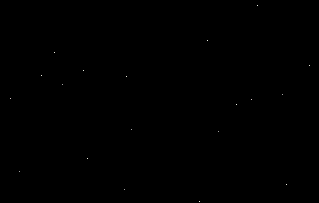
\includegraphics[scale=0.6]{particleFieldZoom}
	\caption{Particle field from the project implementation}
\end{figure}

\subsection{Drawing Lines}
\subsection*{Line Implementation}
\begin{flushleft}
	The line implementation works by starting with two points. The start and
	end of the line. The program will then take these values and calculate 2
	numbers \(d_x\) and \( d_y\). Then, the program will find which axis the
	line moves the most along (Known as the X or Y major). This is done through
	seeing which value between \(d_x\) and \( d_y\) is the greatest. Should \(d_x\)
	be greater we step along the X axis. The same is true should \(d_y\) be greater.
	The program then keeps track of this by saving a `step' variable as the corresponding 
	major.
\end{flushleft}

\begin{flushleft}
	The final step before moving onto deciding which pixels get drawn is to calculate
	the increase required each iteration in the \(x\) and \(y\) directions.
	This increase is found by dividing \(d_x\) and \(dy\) by the step variable that was
	saved earlier. 
\end{flushleft}

\begin{flushleft}
	In order to draw the line the program now iterates over as many `steps'
	needed to draw the line from the start to the end. During each iteration
	the program will check that the pixel is within the bounds of the surface
	and should this check return true the pixel will be drawn. This is done to 
	avoid out of bounds errors within the program. The last stage of the loop is 
	to move to the next pixel in the line by adding the \(x\) and \(y\) increase 
	to our current pixel location.
\end{flushleft}



\begin{figure}[H]
	\centering
	\begin{minipage}[b]{0.4\textwidth}
		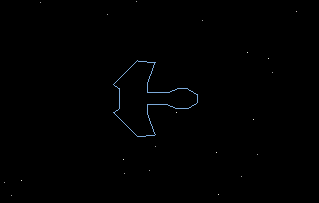
\includegraphics[width=\textwidth]{ship}
		\caption{Ship drawn.}
	\end{minipage}
	\hfill
	\begin{minipage}[b]{0.4\textwidth}
		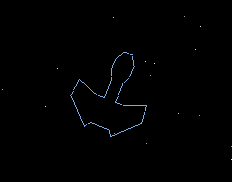
\includegraphics[width=\textwidth]{shipRotate}
		\caption{Ship rotated}
  	\end{minipage}
\end{figure}

\subsection{Drawing Triangles}
\begin{flushleft}
	This algorithm begins by finding the possible bounds of the triangle by 
	iterating through the points given to find the maximum and minimum coordinates. 
	Once the bounds of the triangle are discovered the program will iterate 
	through every pixel within the bounds. Every loop the program will check 
	if the current pixel (\(X\)) is within the triangle by performing 3 half-plane tests.
	These tests are performed using the following algorithm \(F(X)=n \cdot (X - P)\).
	Should \(F(X) > 0\) be true for any of the lines the program continues onto 
	the next pixel. Should the pixel pass all the half-plane tests the program will 
	then check the pixel is within the window and if it is the pixel gets drawn. 

\end{flushleft}

\subsection{Barycentric Interpolation}
\begin{flushleft}
	
\end{flushleft}
\begin{figure}[H]
	\centering
	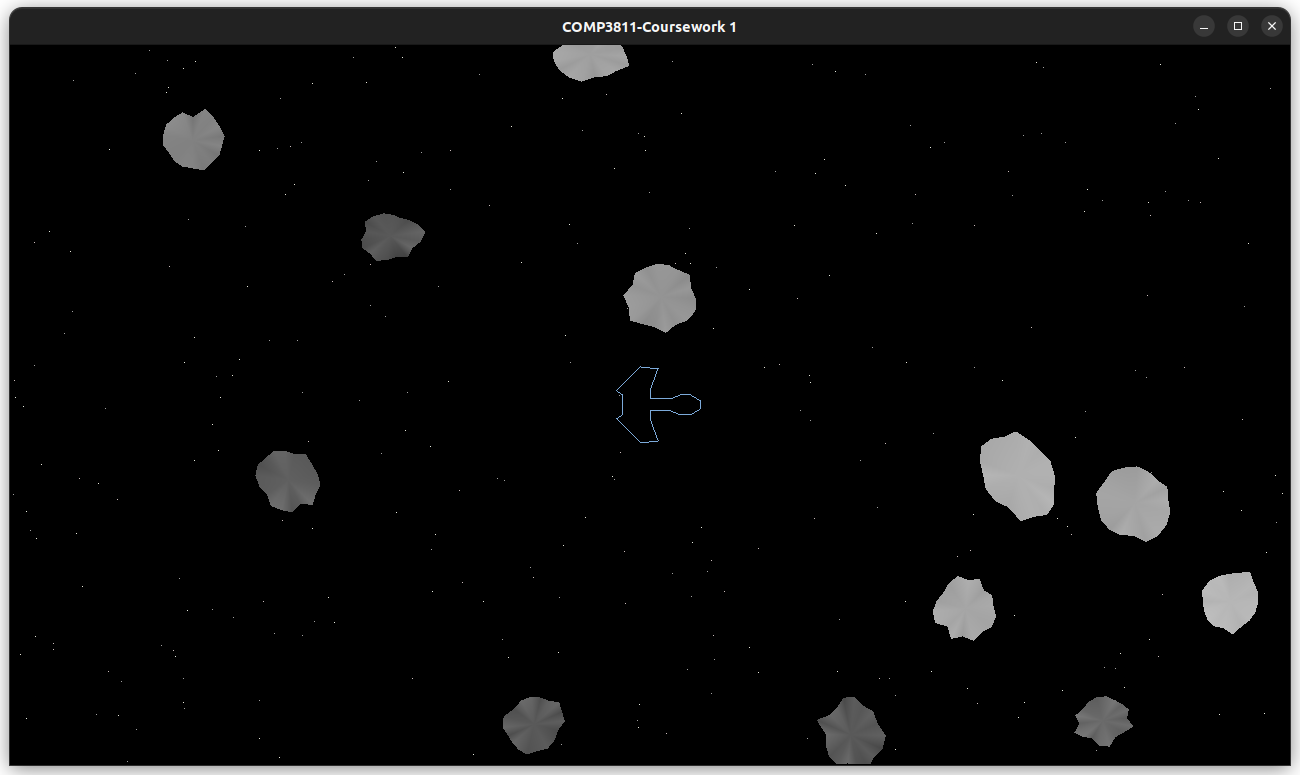
\includegraphics[width=0.6\textwidth]{interpol.png}
\end{figure}

\subsection{Blitting Images}

\subsection{Testing: Lines}

\subsection{Testing: Triangles}

\subsection{Benchmark: Blitting}

\subsection{Benchmark: Line drawing}

\subsection{Your own spaceship}

\subsection*{}
%----------------------------------------------------------------------------------------
%	BIBLIOGRAPHY
%----------------------------------------------------------------------------------------

\printbibliography% Output the bibliography

%----------------------------------------------------------------------------------------

\end{document}